\subsubsection*{Training Insights}
ResNet50V2 training was very similar to the other ResNets with some trainings yielding good results but also many trainings that were not able to pick up useful information from the images. Interestingly, nine out of the ten trainings ended up predicting masses lower than the actual masses, indicated by a positive $\mu$ value. Overall, ResNet50V2 was able to perform quite well on multiple training runs with a $\sigma < 0.15$ on three occasions.

\subsubsection*{Best Performing Model}
The best performing ResNet50V2 model was the second best performing deep learning model overall with a $\sigma < 0.14$. Despite the good sense for the relative masses, the model still predicted lower masses throughout the mass range resulting in a $\mu$ of $0.087$. The training itself did not seem to produce a good performing model at all with high validation losses until almost the end of training. Somehow, the model seemed to detect useful features just before the end of training, resulting in a good performance.

\begin{figure}[H]
\centering
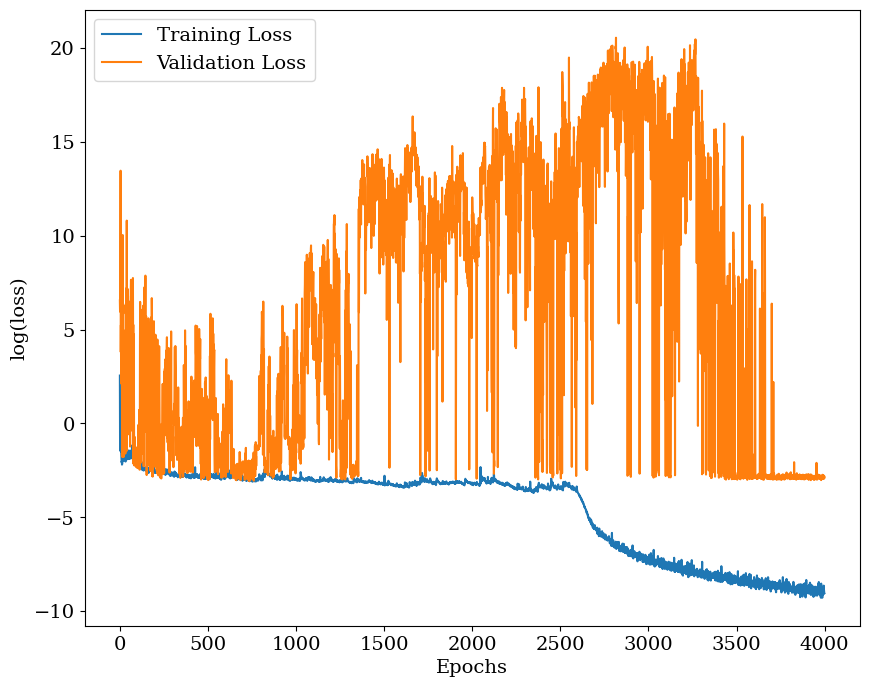
\includegraphics[width=.667\textwidth]{images/Chapter4/Res50V2/resnet50V2_history.png}
\caption{Best performing ResNet50V2 model after ten training runs. Astonishingly, the training was quite poor until the training loss rapidly decreased from epoch 3600 on. The validation loss only settled to a low value just a few hundred epochs before the end of the training. } 
\label{fig:resnet50v2_best_history}
\end{figure}


\begin{figure}[H]
\centering
\begin{subfigure}{.46\textwidth}
  \centering
  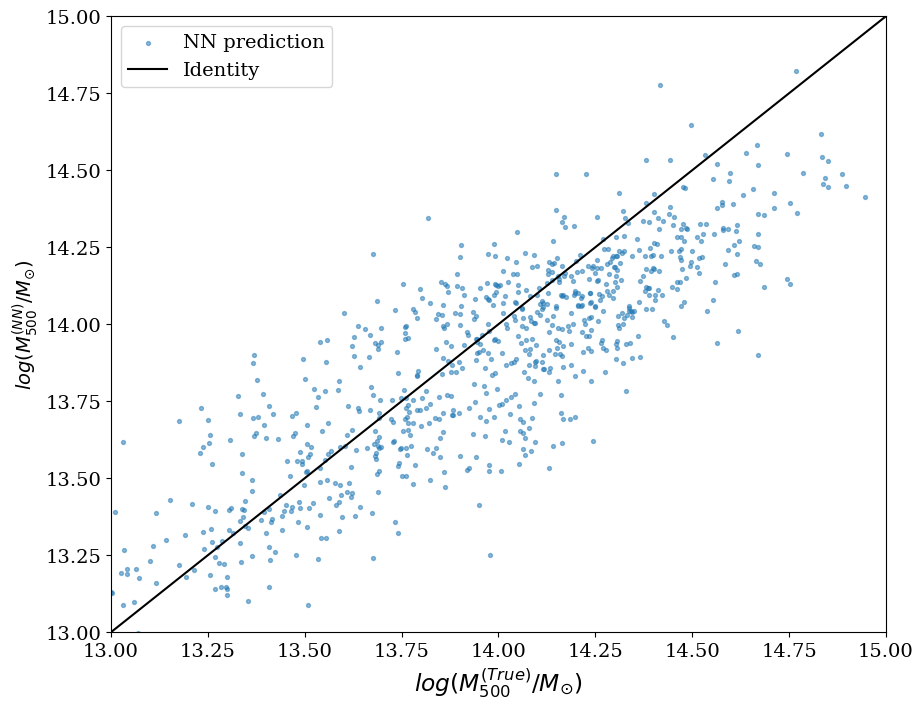
\includegraphics[width=\linewidth]{images/Chapter4/Res50V2/resnet50v2_test.png}
  \caption{Model predictions on the test set.}
  \label{fig:best_perf_resnet50v2_a}
\end{subfigure}%
\hspace{.6em}
\begin{subfigure}{.46\textwidth}
  \centering
  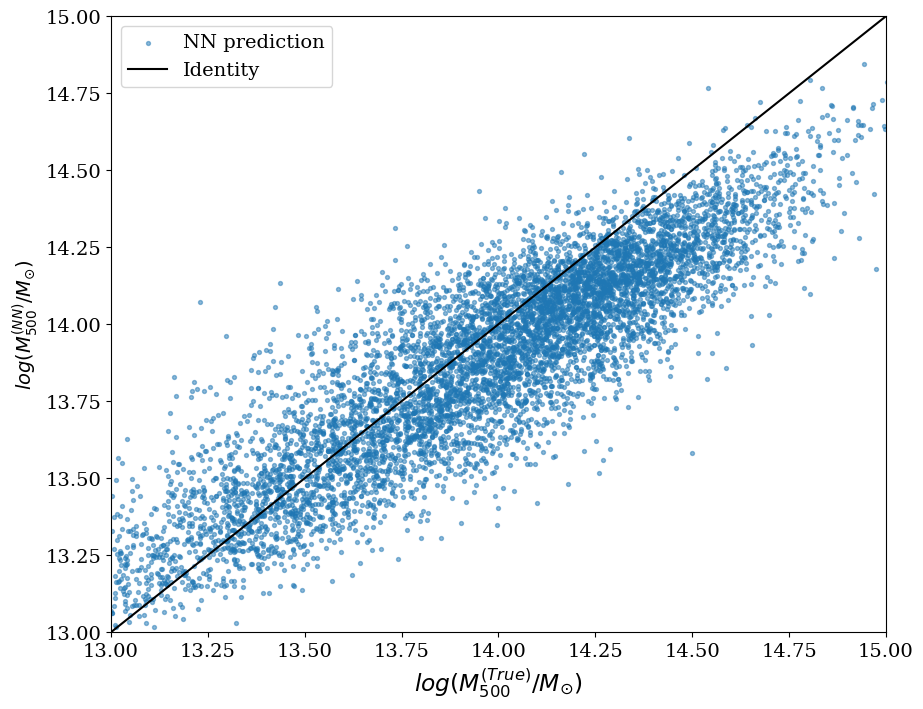
\includegraphics[width=\linewidth]{images/Chapter4/Res50V2/resnet50v2_training.png}
  \caption{Model predictions on the training set.}
  \label{fig:best_perf_resnet50v2_b}
\end{subfigure}
\begin{subfigure}{.46\textwidth}
  \centering
  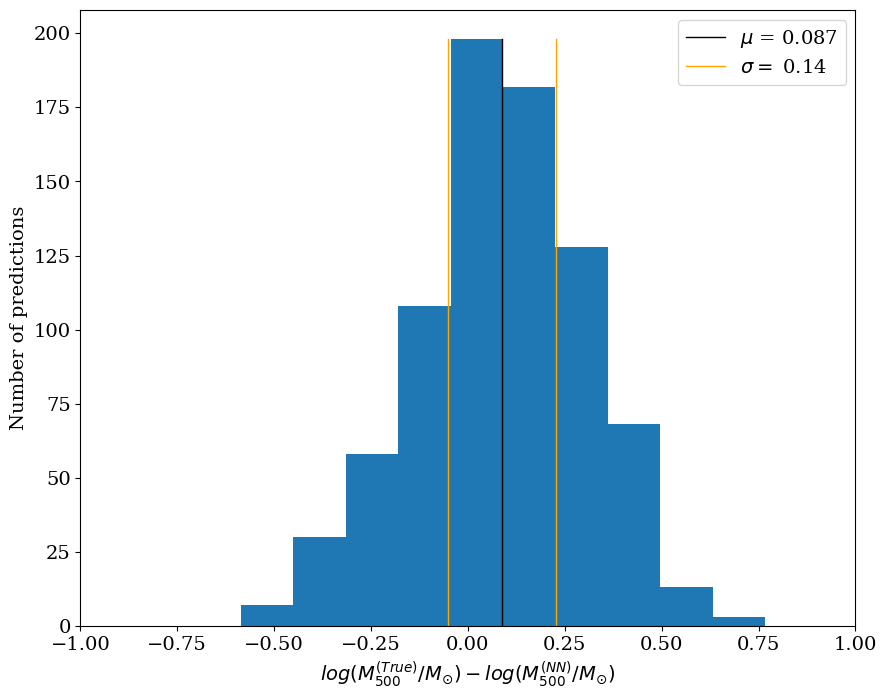
\includegraphics[width=\linewidth]{images/Chapter4/Res50V2/resnet50v2_test_hist.png}
  \caption{Histogram of model predictions on the test set.}
  \label{fig:best_perf_resnet50v2_c}
\end{subfigure}%
\hspace{.6em}
\begin{subfigure}{.46\textwidth}
  \centering
  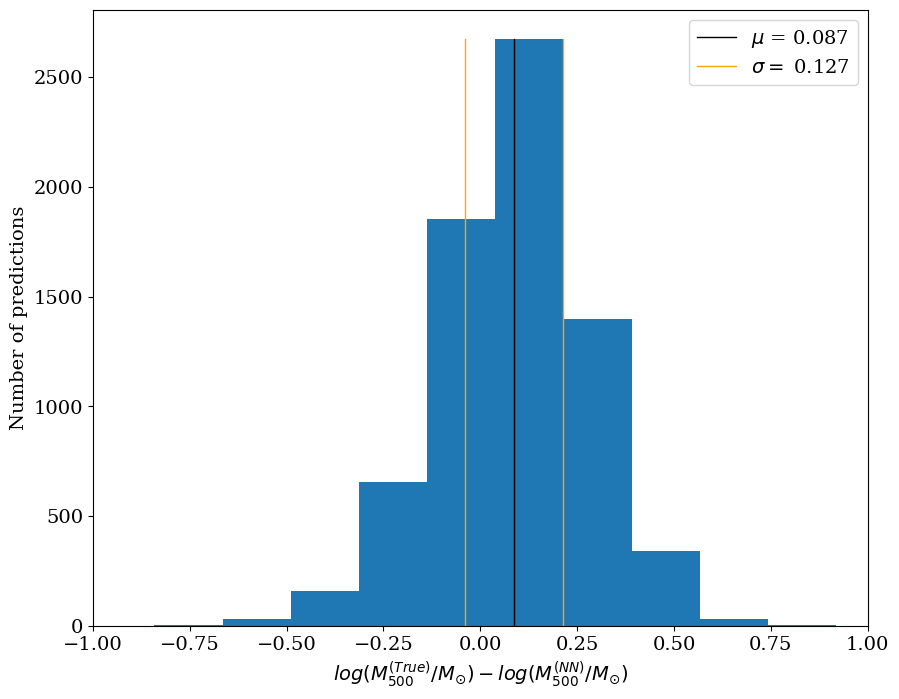
\includegraphics[width=\linewidth]{images/Chapter4/Res50V2/resnet50v2_training_hist.png}
  \caption{Histogram of model predictions on the training set.}
  \label{fig:best_perf_resnet50v2_d}
\end{subfigure}
\caption{Prediction on the test and training set look similar. The standard deviation $\sigma$ on the training set is slightly lower which could be a sign for little overfitting.} 
\label{fig:best_perf_resnet50v2}
\end{figure}

The ResNet50V2 model seems to be quite good at galaxy cluster estimation. It comes close to the basic CNN ($\sigma \sim 0.13$) with a standard deviation of $\sigma \sim 0.14$. With some optimization in training speed, the number of epochs or the input image resolution, I can see this model outperforming the basic CNN in the future. 